\documentclass{standalone}
\usepackage{tikz}
\usetikzlibrary{patterns, positioning}
\usepackage[sfdefault]{ClearSans} %% option 'sfdefault' activates Clear Sans as the default text font
\usepackage[T1]{fontenc}

\begin{document}
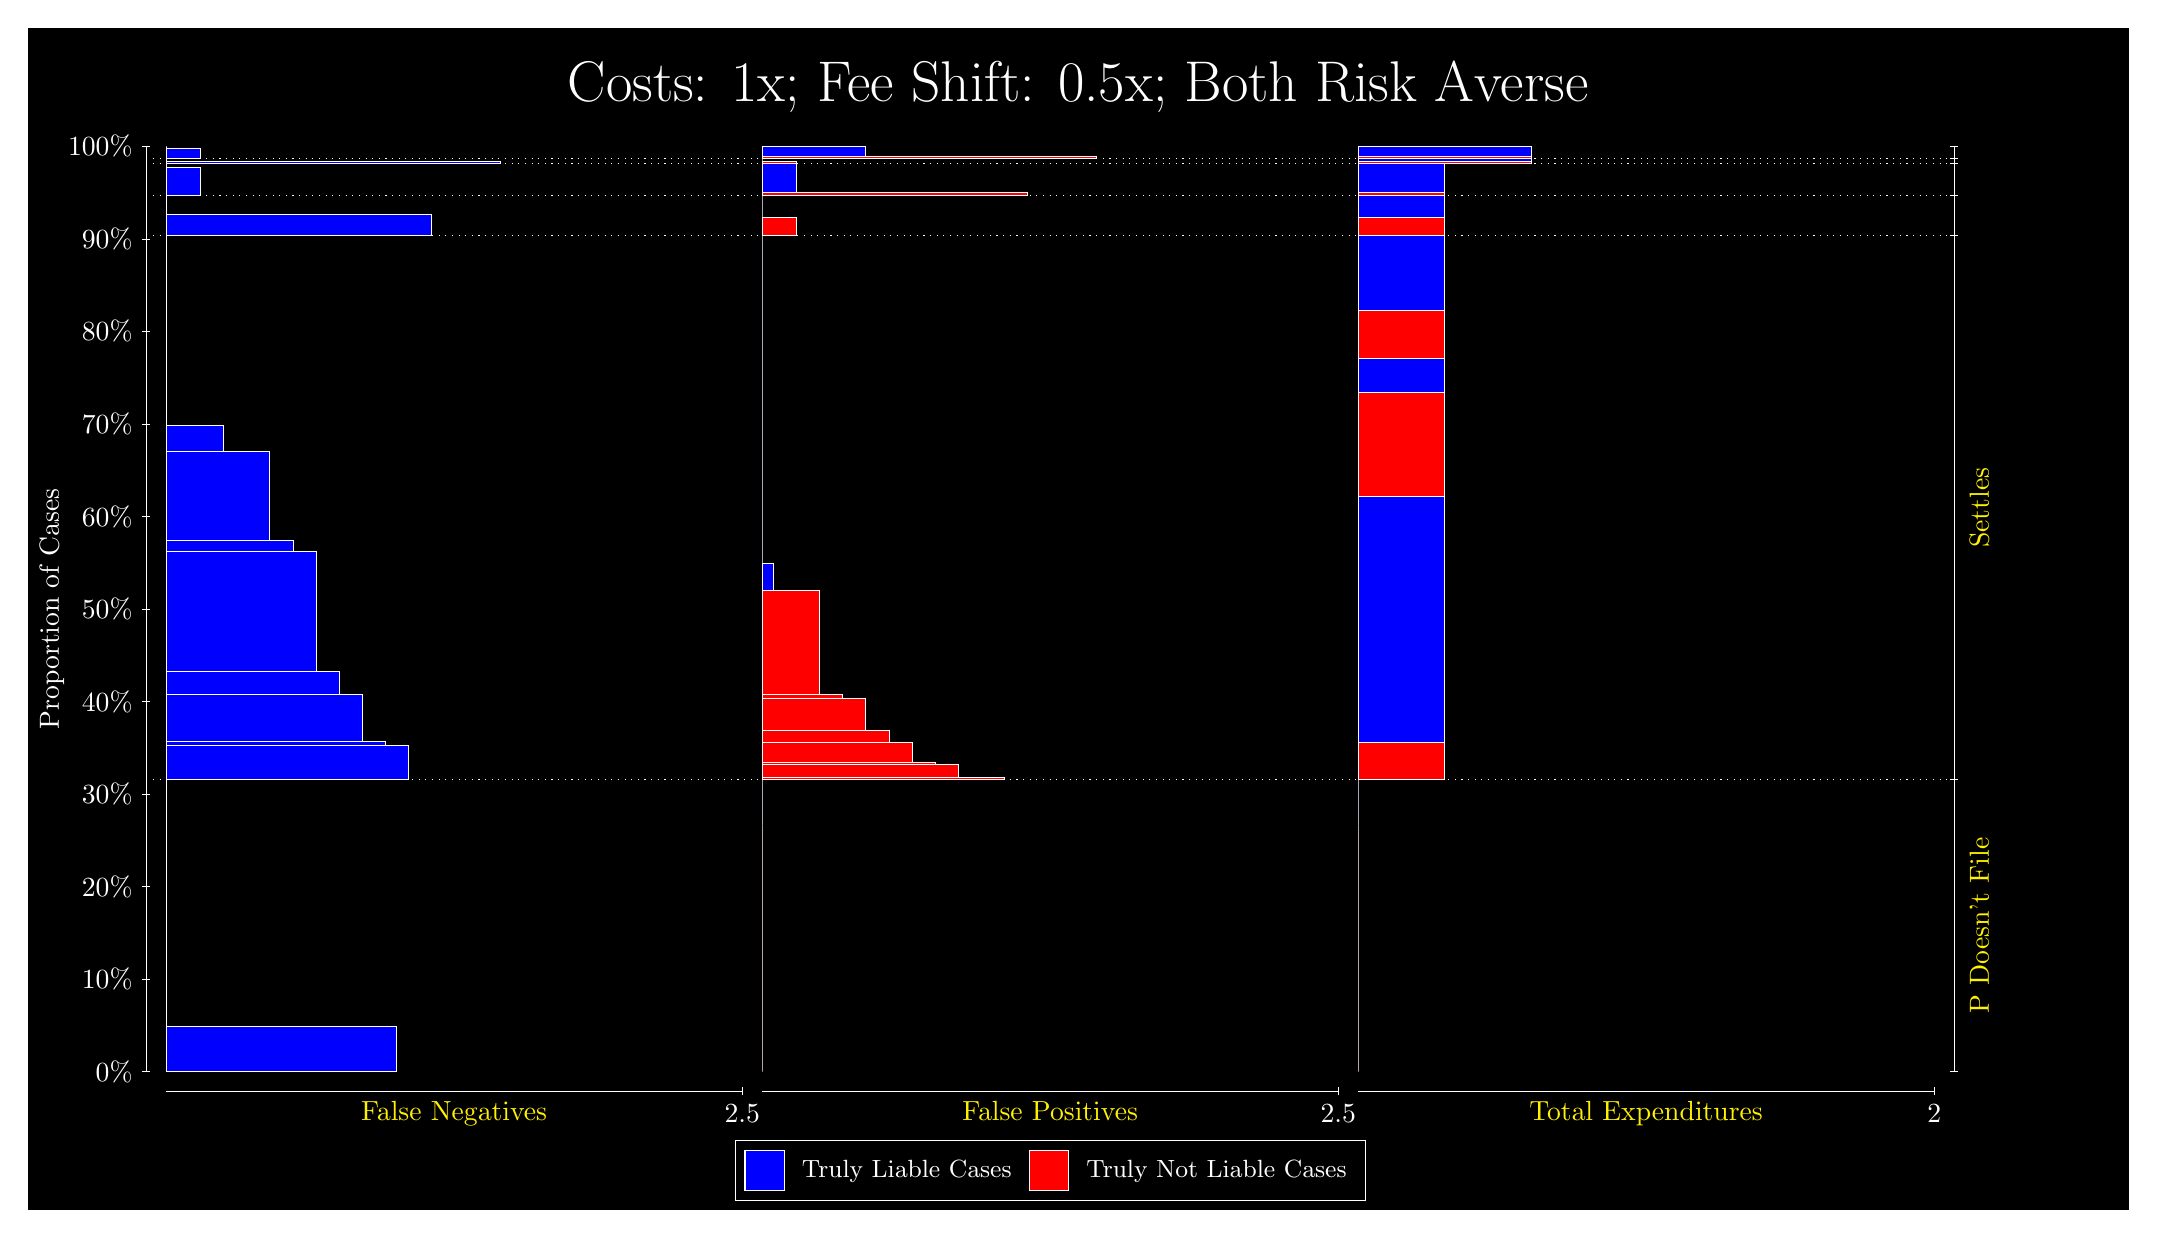
\begin{tikzpicture}
\draw[fill=black] (0,0) rectangle (26.667,15);
\draw[text=white] (0,13.5) rectangle (26.667,15) node[midway] {\huge Costs: 1x; Fee Shift: 0.5x; Both Risk Averse};
\draw[white, very thin] (1.5,1.75) -- (1.5,13.5);
\node[rotate=90, text=white, anchor=center] at (0.3, 7.625) {Proportion of Cases};
\draw[white, very thin] (1.45,1.75) -- (1.55,1.75);
\node[text=white, anchor=east] at (1.45, 1.75) {0\%};
\draw[white, very thin] (1.45,2.925) -- (1.55,2.925);
\node[text=white, anchor=east] at (1.45, 2.925) {10\%};
\draw[white, very thin] (1.45,4.1) -- (1.55,4.1);
\node[text=white, anchor=east] at (1.45, 4.1) {20\%};
\draw[white, very thin] (1.45,5.275) -- (1.55,5.275);
\node[text=white, anchor=east] at (1.45, 5.275) {30\%};
\draw[white, very thin] (1.45,6.45) -- (1.55,6.45);
\node[text=white, anchor=east] at (1.45, 6.45) {40\%};
\draw[white, very thin] (1.45,7.625) -- (1.55,7.625);
\node[text=white, anchor=east] at (1.45, 7.625) {50\%};
\draw[white, very thin] (1.45,8.8) -- (1.55,8.8);
\node[text=white, anchor=east] at (1.45, 8.8) {60\%};
\draw[white, very thin] (1.45,9.975) -- (1.55,9.975);
\node[text=white, anchor=east] at (1.45, 9.975) {70\%};
\draw[white, very thin] (1.45,11.15) -- (1.55,11.15);
\node[text=white, anchor=east] at (1.45, 11.15) {80\%};
\draw[white, very thin] (1.45,12.325) -- (1.55,12.325);
\node[text=white, anchor=east] at (1.45, 12.325) {90\%};
\draw[white, very thin] (1.45,13.5) -- (1.55,13.5);
\node[text=white, anchor=east] at (1.45, 13.5) {100\%};

\draw[white, very thin] (24.457,1.75) -- (24.457,13.5);
\draw[white, very thin] (24.407,1.75) -- (24.507,1.75);
\node[anchor=west] at (24.407, 1.75) {};
\draw[white, very thin] (24.407,5.4572) -- (24.507,5.4572);
\node[anchor=west] at (24.407, 5.4572) {};
\draw[white, very thin] (24.407,12.364) -- (24.507,12.364);
\node[anchor=west] at (24.407, 12.364) {};
\draw[white, very thin] (24.407,12.874) -- (24.507,12.874);
\node[anchor=west] at (24.407, 12.874) {};
\draw[white, very thin] (24.407,13.284) -- (24.507,13.284);
\node[anchor=west] at (24.407, 13.284) {};
\draw[white, very thin] (24.407,13.344) -- (24.507,13.344);
\node[anchor=west] at (24.407, 13.344) {};
\draw[white, very thin] (24.407,13.5) -- (24.507,13.5);
\node[anchor=west] at (24.407, 13.5) {};

\draw[white, very thin, fill=blue] (1.75,1.75) rectangle (4.6775,2.331);
\draw[white, very thin, fill=red] (1.75,2.331) rectangle (1.75,5.4572);
\draw[white, very thin, fill=blue] (1.75,5.4572) rectangle (4.8239,5.8885);
\draw[white, very thin, fill=blue] (1.75,5.8885) rectangle (4.5312,5.9499);
\draw[white, very thin, fill=blue] (1.75,5.9499) rectangle (4.2384,6.5428);
\draw[white, very thin, fill=blue] (1.75,6.5428) rectangle (3.9457,6.8348);
\draw[white, very thin, fill=blue] (1.75,6.8348) rectangle (3.6529,8.3604);
\draw[white, very thin, fill=blue] (1.75,8.3604) rectangle (3.3602,8.4976);
\draw[white, very thin, fill=blue] (1.75,8.4976) rectangle (3.0674,9.6222);
\draw[white, very thin, fill=blue] (1.75,9.6222) rectangle (2.4819,9.9554);
\draw[white, very thin, fill=red] (1.75,9.9554) rectangle (1.75,12.364);
\draw[white, very thin, fill=blue] (1.75,12.364) rectangle (5.1167,12.641);
\draw[white, very thin, fill=red] (1.75,12.641) rectangle (1.75,12.874);
\draw[white, very thin, fill=blue] (1.75,12.874) rectangle (2.1891,13.237);
\draw[white, very thin, fill=red] (1.75,13.237) rectangle (1.75,13.284);
\draw[white, very thin, fill=blue] (1.75,13.284) rectangle (5.9949,13.315);
\draw[white, very thin, fill=red] (1.75,13.315) rectangle (1.75,13.344);
\draw[white, very thin, fill=blue] (1.75,13.344) rectangle (2.1891,13.469);
\draw[white, very thin, fill=red] (1.75,13.469) rectangle (1.75,13.5);
\draw[white, very thin, fill=red] (9.3189,1.75) rectangle (9.3189,4.8762);
\draw[white, very thin, fill=blue] (9.3189,4.8762) rectangle (9.3189,5.4572);
\draw[white, very thin, fill=red] (9.3189,5.4572) rectangle (12.393,5.4908);
\draw[white, very thin, fill=red] (9.3189,5.4908) rectangle (11.807,5.653);
\draw[white, very thin, fill=red] (9.3189,5.653) rectangle (11.515,5.6742);
\draw[white, very thin, fill=red] (9.3189,5.6742) rectangle (11.222,5.9335);
\draw[white, very thin, fill=red] (9.3189,5.9335) rectangle (10.929,6.0901);
\draw[white, very thin, fill=red] (9.3189,6.0901) rectangle (10.636,6.4878);
\draw[white, very thin, fill=red] (9.3189,6.4878) rectangle (10.344,6.5446);
\draw[white, very thin, fill=red] (9.3189,6.5446) rectangle (10.051,7.8654);
\draw[white, very thin, fill=blue] (9.3189,7.8654) rectangle (9.4652,8.1985);
\draw[white, very thin, fill=blue] (9.3189,8.1985) rectangle (9.3189,12.364);
\draw[white, very thin, fill=red] (9.3189,12.364) rectangle (9.758,12.597);
\draw[white, very thin, fill=blue] (9.3189,12.597) rectangle (9.3189,12.874);
\draw[white, very thin, fill=red] (9.3189,12.874) rectangle (12.686,12.921);
\draw[white, very thin, fill=blue] (9.3189,12.921) rectangle (9.758,13.284);
\draw[white, very thin, fill=red] (9.3189,13.284) rectangle (9.758,13.313);
\draw[white, very thin, fill=blue] (9.3189,13.313) rectangle (9.3189,13.344);
\draw[white, very thin, fill=red] (9.3189,13.344) rectangle (13.564,13.375);
\draw[white, very thin, fill=blue] (9.3189,13.375) rectangle (10.636,13.5);
\draw[white, very thin, fill=red] (16.888,1.75) rectangle (16.888,4.8762);
\draw[white, very thin, fill=blue] (16.888,4.8762) rectangle (16.888,5.4572);
\draw[white, very thin, fill=red] (16.888,5.4572) rectangle (17.986,5.9335);
\draw[white, very thin, fill=blue] (16.888,5.9335) rectangle (17.986,9.0541);
\draw[white, very thin, fill=red] (16.888,9.0541) rectangle (17.986,10.375);
\draw[white, very thin, fill=blue] (16.888,10.375) rectangle (17.986,10.806);
\draw[white, very thin, fill=red] (16.888,10.806) rectangle (17.986,11.417);
\draw[white, very thin, fill=blue] (16.888,11.417) rectangle (17.986,12.364);
\draw[white, very thin, fill=red] (16.888,12.364) rectangle (17.986,12.597);
\draw[white, very thin, fill=blue] (16.888,12.597) rectangle (17.986,12.874);
\draw[white, very thin, fill=red] (16.888,12.874) rectangle (17.986,12.921);
\draw[white, very thin, fill=blue] (16.888,12.921) rectangle (17.986,13.284);
\draw[white, very thin, fill=red] (16.888,13.284) rectangle (19.083,13.313);
\draw[white, very thin, fill=blue] (16.888,13.313) rectangle (19.083,13.344);
\draw[white, very thin, fill=red] (16.888,13.344) rectangle (19.083,13.375);
\draw[white, very thin, fill=blue] (16.888,13.375) rectangle (19.083,13.5);
\draw[white, dotted] (1.5,5.4572) -- (24.457,5.4572);
\draw[white, dotted] (1.5,12.364) -- (24.457,12.364);
\draw[white, dotted] (1.5,12.874) -- (24.457,12.874);
\draw[white, dotted] (1.5,13.284) -- (24.457,13.284);
\draw[white, dotted] (1.5,13.344) -- (24.457,13.344);
\draw[white, very thin] (1.75,1.5) -- (9.0689,1.5);
\node[text=yellow, anchor=north] at (5.4094, 1.5) {False Negatives};
\draw[white, very thin] (9.0689,1.45) -- (9.0689,1.55);
\node[text=white, anchor=north] at (9.0689, 1.45) {2.5};

\draw[white, very thin] (9.3189,1.5) -- (16.638,1.5);
\node[text=yellow, anchor=north] at (12.978, 1.5) {False Positives};
\draw[white, very thin] (16.638,1.45) -- (16.638,1.55);
\node[text=white, anchor=north] at (16.638, 1.45) {2.5};

\draw[white, very thin] (16.888,1.5) -- (24.207,1.5);
\node[text=yellow, anchor=north] at (20.547, 1.5) {Total Expenditures};
\draw[white, very thin] (24.207,1.45) -- (24.207,1.55);
\node[text=white, anchor=north] at (24.207, 1.45) {2};

\node[text=yellow, centered, rotate=90] at (24.777, 3.6036) {P Doesn't File};
\node[text=yellow, centered, rotate=90] at (24.777, 8.9104) {Settles};





\draw (12.978300999999998,1.5) node[draw=none] (baseCoordinate) {};
\begin{scope}[align=center]
        \matrix[scale=0.5, draw=white, below=0.5cm of baseCoordinate, nodes={draw}, column sep=0.1cm]{
            \node[rectangle, draw, minimum width=0.5cm, minimum height=0.5cm, fill=blue] {}; &
            \node[draw=none, font=\small, text=white] (B) {Truly Liable Cases}; &
            \node[rectangle, draw, minimum width=0.5cm, minimum height=0.5cm, fill=red] {}; &
            \node[draw=none, font=\small, text=white] (B) {Truly Not Liable Cases}; \\
            };
\end{scope}

\end{tikzpicture}
\end{document}